% \documentclass{minimal}
% \usepackage{tikz}

% \begin{document}
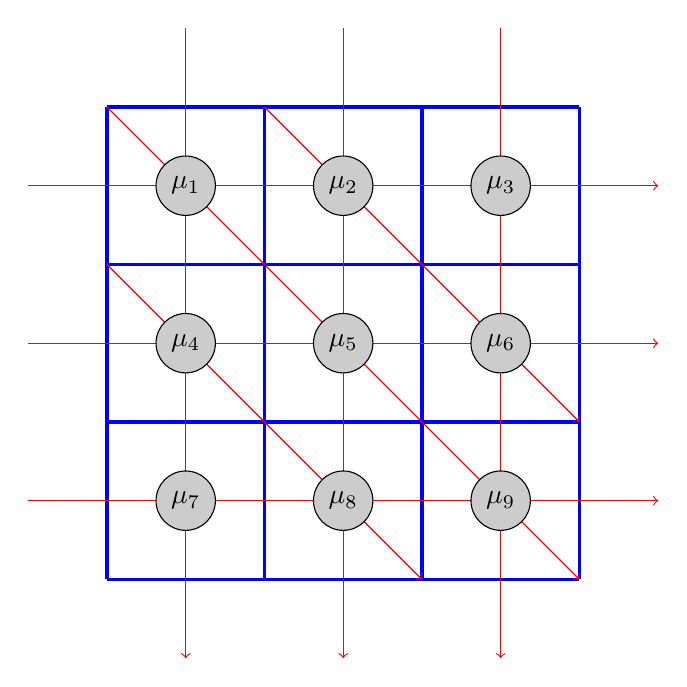
\begin{tikzpicture}[darkstyle/.style={circle,draw,fill=gray!40,minimum size=20}]

    \newcommand*{\cellsize}{2}%
    \newcommand*{\numcells}{3}%
    \newcommand*{\arrowoffset}{(1/2)}%

    \draw [step=\cellsize, blue, very thick] (0,0) grid ({\cellsize*\numcells},{-\cellsize*\numcells});


    % horizontal ↓
    \foreach \i in {0,...,2}
        \draw[red, ->] ({-\arrowoffset * \cellsize}, {-(\i + 1/2) * \cellsize})
        -- ({(\numcells + \arrowoffset) * \cellsize}, {-(\i + 1/2) * \cellsize}) ;

    % vertikal ↓
    \foreach \i in {0,...,2}
        \draw[red, ->] ({(\i + 1/2) * \cellsize}, {\arrowoffset * \cellsize})
        -- ({(\i + 1/2) * \cellsize}, {-(\numcells + \arrowoffset) * \cellsize}) ;

    % diagonal [WIP] ↓
    % \foreach \i in {0,...,2}
    %     \draw[red, ->] (0, {-(\i - 1) * \cellsize})
    %     -- ({(\numcells) * \cellsize}, {-(\numcells + \i - 1) * \cellsize}) ;

    % diagonal (manual) ↓
    \draw[red, ->] (0,0) -- ({\numcells * \cellsize},{-(\numcells * \cellsize)}) ;
    \draw[red, ->] (0,-1 * \cellsize) -- ({(\numcells-1) * \cellsize},{-(\numcells * \cellsize)}) ;
    \draw[red, ->] (1 * \cellsize,0) -- ({\numcells * \cellsize},{-((\numcells-1) * \cellsize)}) ;

    % \foreach \i in {0,...,2}
    %     \draw[red] (0,{-2 * \cellsize + \i})--({3 * \cellsize},{1 * \cellsize + \i}) ;


%   \foreach \x in {0,...,\numcells}
%     \foreach \y [count=\yi] in {0,...,\numcells}
%       \draw (\x\y)--(\x\yi) (\y\x)--(\yi\x) ;

    \foreach \x in {0,...,2}
        \foreach \y in {0,...,2}
            {\pgfmathtruncatemacro{\label}{\numcells * \y + \x + 1}
            \node [darkstyle]  (\x\y) at ({(\x + 1/2) * \cellsize},{-(\y + 1/2) * \cellsize}) {$\mu_{\label}$};}

\end{tikzpicture}
% \end{document}
